% 	    %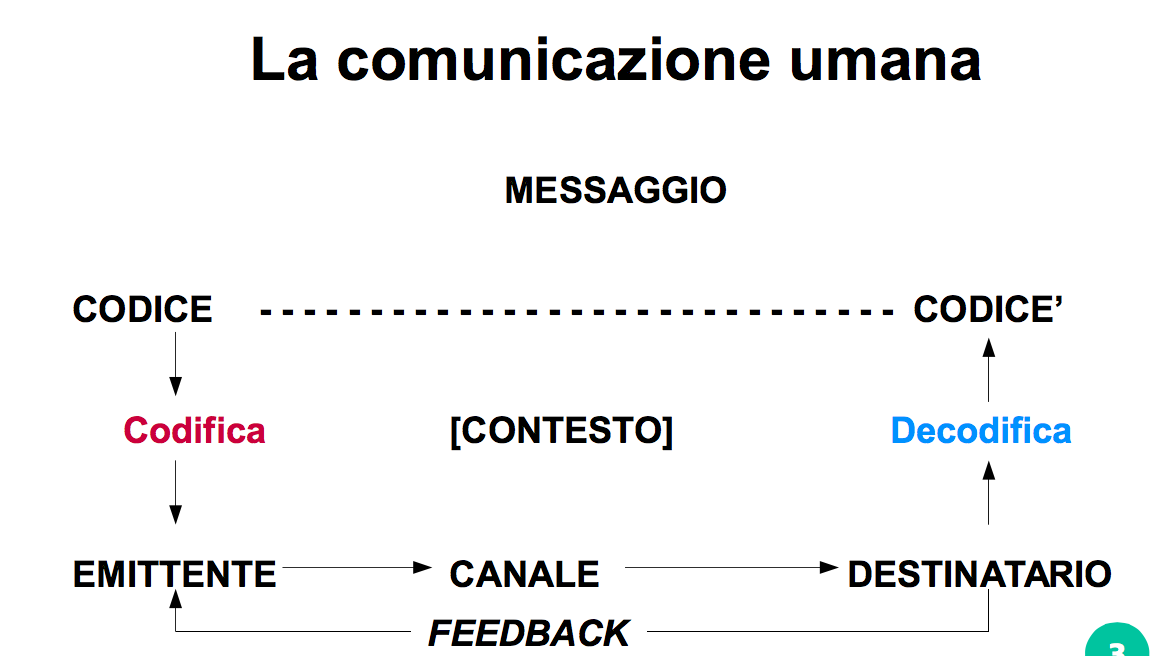
\includegraphics[width=.5\textwidth]{../imgs/comunicazioneUmana.png}
% definizione di segre
% definizione di tito orlandi

\begin{frame}
	\frametitle{Modellare il testo}
	\framesubtitle{Il testo come oggetto del dominio di studio}
	\addtocounter{nframe}{1}

	\begin{block}{Informatica nelle scienze umane}
		L'informatica umanistica ruota attorno alla rappresentazione e all'elaborazione degli oggetti che costituiscono il dominio delle discipline umanistiche.
	\end{block}

	\begin{block}{Testo come oggetto di studio}
		Il testo è tra questi, l'oggetto più ricorrente
	\end{block}

\end{frame}

\begin{frame}
	\frametitle{Modellare il testo}
	\framesubtitle{qual è la natura del testo?}
	\addtocounter{nframe}{1}

	\begin{block}{Modellare il testo}
		Per trattare e rappresentare il testo in ambiente digitale, bisogna formulare un suo modello
	\end{block}

	\begin{block}{Modello del testo}
		Un efficace modello del testo non può prescindere da una determinazione di cosa si intenda per testo e la sua natura. Il fatto è che la rappresentazione (e a maggior ragione l’elaborazione) informatica è ontologicamente formale in senso stretto (Ciotti).
	\end{block}

\end{frame}

\begin{frame}
	\frametitle{Modellare il testo}
	\framesubtitle{Testo: oggetto complesso}
	\addtocounter{nframe}{1}

	\begin{block}{Cos'è il testo}
		Il testo è un oggetto complesso in quanto è in grado di veicolare significato su più livelli strutturali (logico, ontologico, linguistico, autoriale, editoriale, fisico, etc), anche attraverso l’instaurazione di molteplici relazioni tra più livelli.
	\end{block}

	\begin{block}{Ma..}
		Non possediamo nessuna teoria sufficientemente completa del testo
	\end{block}

\end{frame}

\begin{frame}
	\frametitle{Modellare il testo}
	\framesubtitle{Testo: oggetto complesso}
	\addtocounter{nframe}{1}

	\begin{block}{Cos'è il testo}
		Si tratta di una entità informativa complessa. in quanto è il prodotto di più agenti e più fattori
	\end{block}

\end{frame}

\begin{frame}
	\frametitle{Modellare il testo}
	\framesubtitle{Tentativo..}
	\addtocounter{nframe}{1}

	\begin{block}{Cos'è il testo}
		Il termine ``testo''  si riferisce a un oggetto plurale, in cui esiste
		\begin{itemize}
			\item un livello astratto: la sequenza verbale, la quale a sua volta genera una serie di livelli di contenuti semantici.
			\item un livello materiale: il supporto e le tracce d’inchiostro
			\item un livello dinamico: il testo viene creato da un autore e ricreato dal lettore
		\end{itemize}

	\end{block}

\end{frame}

% Molteplici teorie del testo, quasi tutte sbilanciate sul livello verbale-semantico (linguistica testuale)

\begin{frame}
	\frametitle{Modellare il testo}
	\framesubtitle{Definizioni}
	\addtocounter{nframe}{1}

	\begin{block}{Il testo}
		dal latino textum, participio passato di texere ``tessere'' quindi un testo è un ``tessuto'', un ordito di unità di significato (monemi) veicolato da simboli (grafemi)
	\end{block}

\end{frame}

\begin{frame}
	\frametitle{Modellare il testo}
	\framesubtitle{Definizioni}
	\addtocounter{nframe}{1}

	\begin{block}{Il testo secondo Segre 1985}
		Il testo è dunque una successione fissa di significati grafici. Questi significati sono poi portatori di significati semantici.
	\end{block}

\end{frame}

\begin{frame}
	\frametitle{Modellare il testo}
	\framesubtitle{Definizioni}
	\addtocounter{nframe}{1}

	\begin{block}{Il testo secondo Tito Orlandi 2010}
		La produzione di un'attività linguistica intesa in senso stretto, cioè in una delle lingue storicamente date, secondo il concetto saussuriano di langue che produce la parole. Il fatto che essa sia finalizzata a trasmettere un messaggio, pur importante in sé, non interessa per il momento se non marginalmente.
	\end{block}

	\begin{block}{Ancora Tito Orlandi}
		Il Testo si presenta al lettore sotto la forma di rappresentazione di un'espressione linguistica, e poiché l'attività linguistica è multiforme, potrà essere una rappresentazione puramente mentale, astratta, ovvero fonica (verbale), ovvero grafica.
	\end{block}


\end{frame}

\begin{frame}
	\frametitle{Modellare il testo}
	\framesubtitle{Definizioni}
	\addtocounter{nframe}{1}

	\begin{block}{Testo}
		il testo è una entità astratta invariante, che in ogni operazione di realizzazione materiale della sequenza di simboli grafici determina la struttura fisica di un oggetto sensibilmente concreto (ovvero capace di attivare uno dei canali recettivi dell’uomo verso stimoli esterni).
	\end{block}

	\begin{block}{Documento}
		L'oggetto materiale, sensibile, concreto che costituisce il supporto, stabile e riproducibile dell’informazione testuale lo chiamiamo documento.
	\end{block}


\end{frame}




% Possiamo concludere che il testo è l’invariante, la successione di valori, rispetto alle variabili dei caratteri, della scrittura.




% A questa struttura rigida del codice nell’ambito informatico (codice binario) va confrontata la complessa intersezione di codici che costituiscono un testo (da memorizzare).



% Testo vs Documento

% oltre alla sequenza di grafemi, a un testo nel senso da noi indicato possono essere ascritte anche le segmentazioni logiche e le partizioni interne di interi blocchi
% il testo ha una certa struttura, i cui elementi sono determinati dalla struttura logico semantica del discorso

% esiste anche un modello documento
% possibilità significative che derivano da una semantizzazione esplicita degli elementi non verbali di un testo scritto.
% ruolo della disposizione tipografica e topografica del segno grafico nella pagina bianca

% quale concezione o modello ontologico del testo è implicata nella rappresentazione informatica?

% natura del testo: il testo è, in un senso importante, una “ordered hierarchy of content objects (OHCO)”, una gerarchia ordinata di oggetti di contenuto [DeRose et al., 1990:3]. Gli oggetti di contenuto testuale a cui si fa riferimento in questa teoria sono sostanzialmente le strutture editoriali astratte di cui si com- pone un testo. Essi sono gerarchici poiché alcuni degli oggetti testuali con- tengono altri, e ordinati in quanto esiste una relazione lineare tra due oggetti posti sul medesimo livello gerarchico.

% il genere determina gli elementi che costituiscono il testo, quindi il tipo di documento. Reciprocamente un genere testuale è individuato dalla classe di oggetti di contenuto che contiene.
% Su questo impianto teorico si è basata, ad esempio, la prima fase del lavoro della Text Encoding Initiative.
% Sono però stati riscontrati una serie di problemi di rappresentazione che costituiscono dei veri e propri controesempi. Ci sono moltissimi casi in cui non esiste assolutamente accordo tra gli specialisti dei testi nell’asserire l’appartenenza di un dato testo a un tipo piuttosto che a un altro.  Questi diversi insiemi di elementi di contenuto non possono essere ricondotti a una struttura gerarchica unitaria.

% classi di elementi testuali che si sovrappongono rompendo i confini della struttura gerarchica di un documento: esempio: struttura metrica e quella morfosintattica di un testo poetico.. (Esempio clavius righe e sentence). Questi elementi si comportano come se appartenessero a diverse gerarchie di oggetti testuali che si sovrappongo.
% Prospettiva analitica:  “ogni prospettiva analitica su un testo determina una struttura gerarchica di oggetti di contenuto”.
% Un corollario operativo di questa tesi è che se due elementi a e b si sovrappongono, allora essi appartengono a due diverse prospettive analitiche.

% Ma è vero che a ogni coppia di elementi che si sovrappongono cor- rispondono due distinte prospettive teoriche? occorrenza di alcuni oggetti testuali che, pur appartenendo ragionevolmente a una medesima pro- spettiva analitica si sovrappongono.
%Se due oggetti testuali evidenziati da una prospettiva teorica si sovrap- pongono, allora essi appartengono rispettivamente a due sottoprospet- tive diverse della prospettiva teorica principale. Questa ultima revisione della teoria gerarchica abbandona qualsiasi assunto di tipo essenzialista. In questa ottica il testo diventa un sistema a più livelli, che corrispondono a diversi punti di vista dell’osservatore.
% • il testo è un oggetto reale dotato di una sua struttura che corrisponde alla struttura del linguaggio di rappresentazione;
% • la struttura o meglio le strutture del testo sono strutture gerar- chiche: le sottoprospettive, comunque esse siano definite, dan- no luogo a gerarchie.

% Alcune teorie avanzano la necessità di abbandonare l’assunto ontologico che il testo sia un oggetto reale del mondo, dotato di una struttura intrinseca: Il testo è dunque una entità che viene costruita e non scoperta e a- nalizzata dalla attività scientifica. soluzione interessante e intellettualmente stimolante alle aporie determinate dal- la teoria gerarchica del testo, specialmente nella tematizzazione del ruolo dell’osservatore nei processi di rappresentazione.

% cos'è il testo (uso comune):
%a) un documento materiale composto da fogli di carta rilegati (o spillati o semplicemente raccolti insieme da un nastro di carta) che contengono tracce di inchiostro variamente disposte (oltre a eventuali tracce di altri materiali)
%b) un discorso linguistico fissato tramite la scrittura su un docu- mento materiale
%c) un’opera dell’ingegno che viene costituita da quel discorso

% cos'è un testo (uso più specialistico)
% d) lo stato linguistico di un singolo testimone materiale di un’opera
% e) lo stato linguistico di un medesimo testimone di un’opera che presenta diverse lezioni identificabili
% f) una versione edita di un’opera
% g) una sequenza coerente di enunciati in una lingua naturale
% Teso è l'invariante rispetto ai segni, è la succesione di valori invariabili. Il testo, dunque è ciò che permane, l’invariante, in ogni operazione di riproduzione materiale della sequenza di simboli grafici.
% Questa definizione di testo come un oggetto astratto allografico sembra fornire un criterio di individuazione di un testo in base al prin- cipio di identità per sostituzione

%OHCO: alla do- manda che cosa è un testo veramente rispondiamo che un testo è un oggetto linguistico astratto organizzato secondo una struttura gerar- chica ordinata di oggetti di contenuto. (Asserzione poi rilevatasi fallace). Ma l’idea di una preminenza della struttura gerarchica nella testualità ha mantenuto un ruolo descrittivo ed esplicativo essenziale.